\section{3D Merging}
\label{3d_merigng}

 
The general goal of electron transmission imaging techniques such as Electron Crystallography, Tomography or Single Particle reconstruction is to gain a 3D computer model by integrating sets of 2D data recorded by an electron microscope. The common mathematical tool that all these techniques share is the Central Section Theorem. \\
The theorem states that the projection along the $z$ direction of a three dimensional volume contains the same information as the central slice in the reciprocal space $(z^*=0)$ of the 3D-Fourier transform of the volume. This means that we can gain a full sampling of the Fourier Transform of the object by the projections along all spatial directions. Accordingly, the 3D reconstruction become just a Inverse Fourier transform. The theory of Electron Optics allows to some approximation the use of images recorded by a Transfer Electron Microscope (TEM) as a projection of the sample. This means that with sufficient images of samples imaged in different orientation to the electron beam, one can simulate the sample's three dimensional density distribution. \\
We have seen in section \autoref{sec:single_image_processing} that the Fourier transform can be used to harvest the repeating signal of the 2D crystal. But since we are dealing with 2D crystals the periodicity is limited to the x,y-plane. The crystal is ideally only formed by one layer in the vertical direction. This results in continuously distributed Fourier component in vertical direction as illustrated in \autoref{fig:lattice_line}. The diffraction spots we have seen in 2D with the index 
$(h,k)$ now become so called \textit{lattice lines} $(h,k,z^*)$ where $h$ and $k$ still correspond to the same Miller index, but $z*$ defines the position along the lattice line. \\
Projections of tilted 2D crystals now produce diffraction spots, where each reflection corresponds to the lattice line $h,k$ and height $z^*$. The height corresponds to the intersection of the tilted plane with the lattice line $h,k$ and thanks to the central section theorem this can be calculated from the tilt geometry of the crystal. So each recorded image produces a set of amplitude and phases with the coordinates $(h,k,z^*)$. The goal is now to densely sample the lattice lines by integrating as much data as possible with varying orientation and tilt angle. This allows us to sample the Fourier transform of our crystal to a certain degree, but due to instrumental restrictions of the TEM, where can not record an image of a any specimen tilted higher than $\pm 70^{\circ}$ there will always be a missing cone.
	
	\begin{figure}
		\centering
		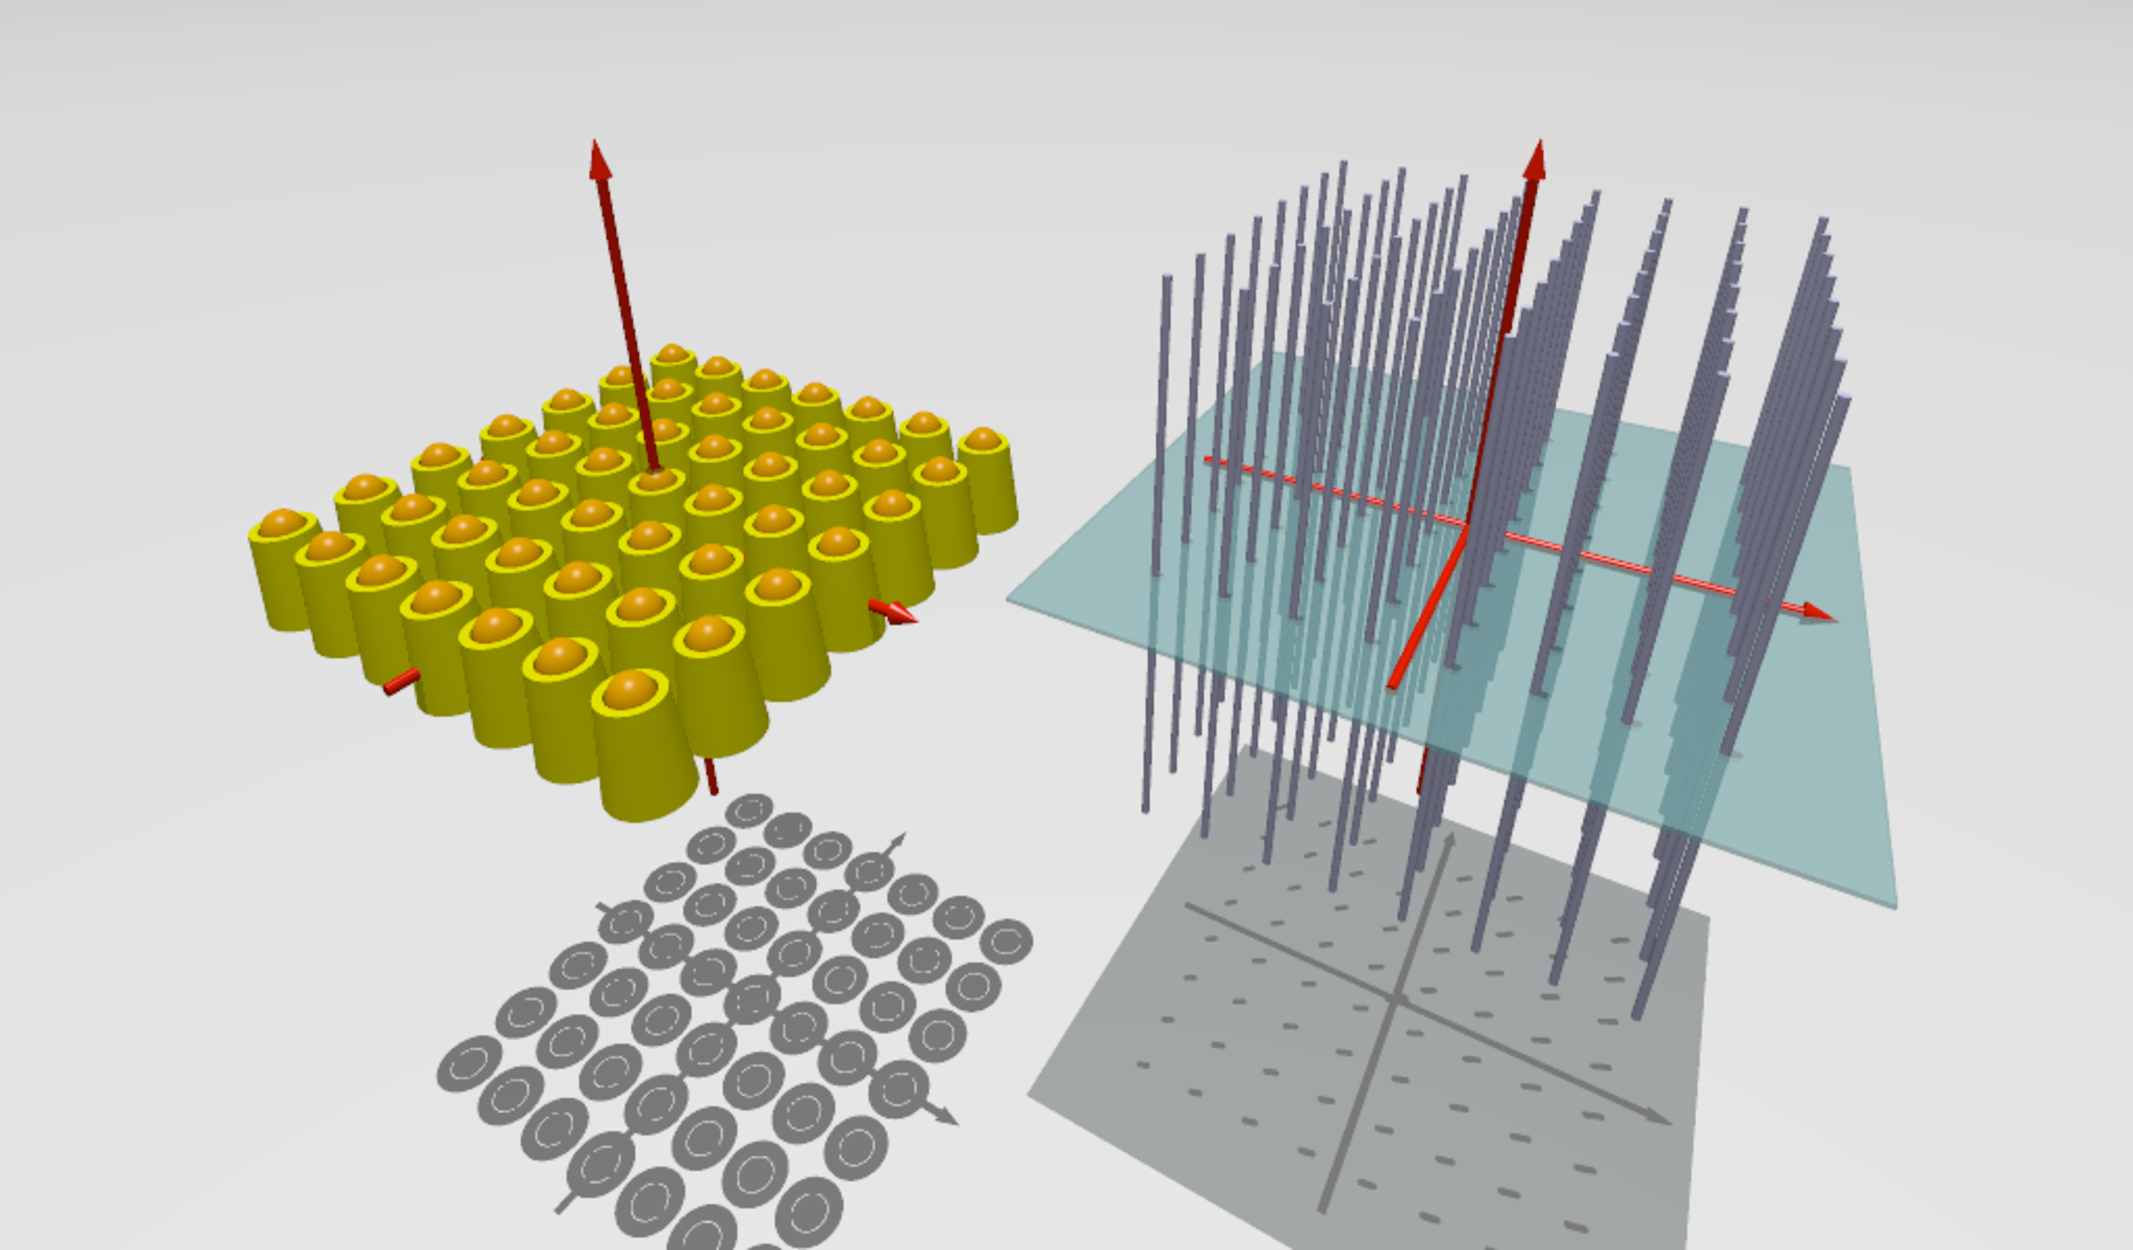
\includegraphics[width=1.0\textwidth]{lattice_line.pdf}
		\caption{The 3D Fourier transform of a 2D crystal forms so called lattice lines perpendicular to the x,y-plane.}
		\label{fig:lattice_line}
	\end{figure}


\subsection{3D Merigng in {\twodx}}
\label{3d_merigng_2dx}

 3D merging in {\twodx} in follows the same workflow as for 2D merging. The problem is still merging data from different images into one common data set. Therefore finding the common phase origin is the task at hand. But in contrast to 2D data  where each reflection $h,k$ had a height $z^*=0$, the amplitude and phases of a tilted sample are usually associated with a reflection at a height that is not zero. These measurements belong to a tilted plane in the 3D Fourier space, where the tilt geometry is defined by the tilt angle (\textit{TANGL}) and the orientation of the lattice on that plane (\textit{TAXA}). If we would now try to refine the phase origin of the tilted image data with non-tilted dataset, then the data points available for comparison would only be the one that lie on the tilt axis. Those measurements are to few to give a sufficient alignment of the tilted data. To deal with the alignment problem of the first tilted data we need to increase the range in $z*$ direction, so that a wider region for allowed comparisons between the non-tilted and the reference data exists as illustrated in \autoref{fig:zstarwin}. \\

	\begin{figure}[H]
		\centering
		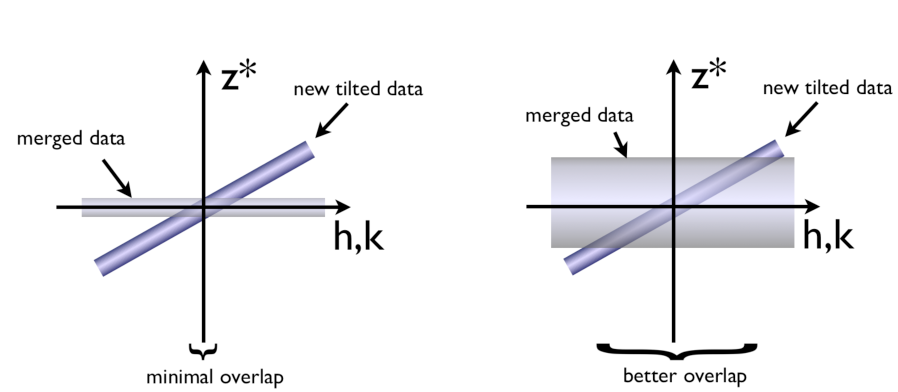
\includegraphics[width=1.0\textwidth]{zstarwin.pdf}
		\caption{The alignment of data from tilted sample when the reference only consists of data from non-tiled sample is almost impossible, since the only data for comparison lie in the tilt axis (left). In this case the vertical tolerance range for comparisons has to be enlarged, which allows more comparisons (right).}
		\label{fig:zstarwin}
	\end{figure}

In the following steps we will show how {\twodx}\texttt{\_merge} can merge data from 2D crystals with different tilt geometry to a 3D reconstruction of your protein structure.  
\begin{enumerate}
	\item We advise you to always  backup your project before you start with 3D Merging, using the custom script \textit{Synchronize with Backup}. This script allows you to submit your project data to a different directory. This is described in more detail in \autoref{sec:sync_project}.
	\item Also save the merged map from 2D merging with help of the \textit{Copy Merged Dataset}\index{Copy Merged Dataset} custom script. This script allows you to copy the last merging result to any of the given 10 registers as illustrated in \autoref{fig:2dx_merge_merged_map_3d}.  Add a comment to the register so you will recognize the merged result in the future.
	\begin{figure}[H]
		\centering
		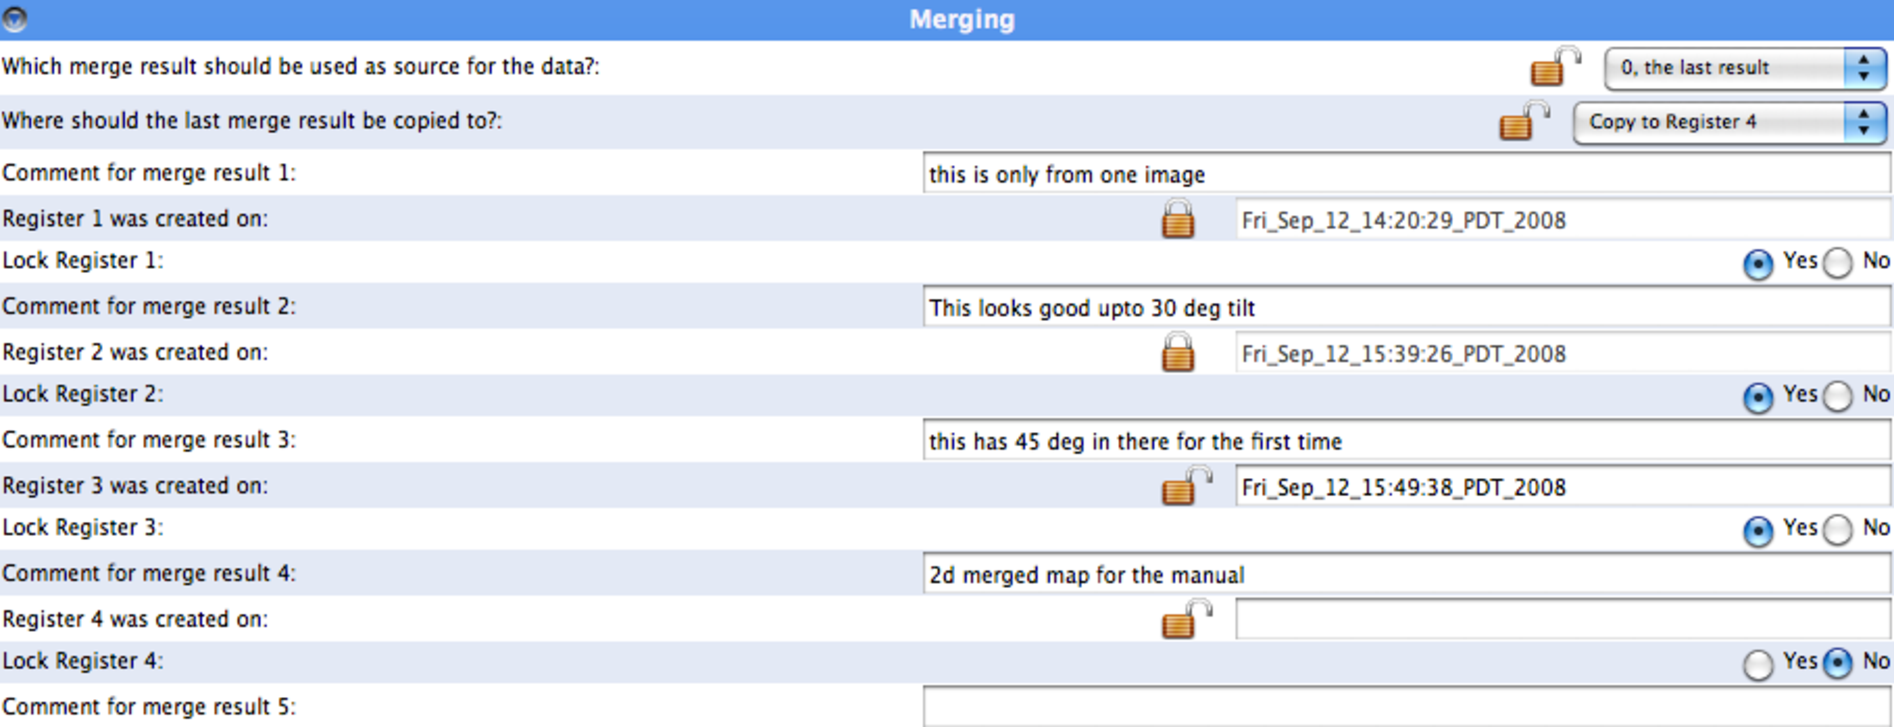
\includegraphics[width=1.0\textwidth]{2dx_merge_merged_map.pdf}
		\caption{Saves the merging result to the selected register. This register can then also be selected as a reference at a later point.}
		\label{fig:2dx_merge_merged_map_3d}
	\end{figure}
	
	\item To let {\twodx}\texttt{\_merge} know that we are about to merge in three dimensions switch the \textit{Modus of Merging}\index{Modus of Merging!3D} to \textit{3D} in the Parameter panel.
	\item Select all processed images that belong to the lowest tilt group ($TANGL \leq 30$), except the non-tilt data. Preferably, the selection should include ten or more projections with reliable measurements. As we have learned in \autoref{sec:det_tilt}, the projections of sample with low tilt is determined by defocus gradient which can be unreliable to some extent, therefore it is essential that the handedness is correct.
	\item We have mentioned the critical step of aligning the first tilted dataset to a 2D merged map. So before running \textit{Refine Once}\index{Refine Once!3D} limit the selected tilted data set to 15 \AA~with the parameter \textit{RESMAX}. In this first 3D refinement step it is indispensable to have sufficient reference points ($>20$) for the phase origin determination. This can be reached by increasing vertical $z^*$ tolerance along a lattice line, which is defined by the processing parameter \textit{3D: zstarwin} in the 3D Merging section. In the beginning of 3D merging set this parameter to 0.2 or something higher. This measure depends on the vertical thickness of your crystal defined by the parameter \textit{ALAT}. When refining the highest tilt data  \textit{zstarwin}\index{zstarwin} should be decreased to $\frac{1}{2*ALAT}$. So for a 200 \AA~sample we eventually set \textit{zstarwin} to 0.0025, just to give you a feeling for the value range. 
	\item As in 2D merging we start out with a step size of 6.0 (\textit{Stepsize of the phase origin search} )and 60 steps (\textit{Number of steps in the phase origin search}).
	\item \label{sec:refine_once_3d} Run \textit{Refine Once} until the phase origins do not essentially change anymore.
	\item Examine the refinement of the tilted data to the non-tilted by looking at the \texttt{origtilt} output \textit{LOG: origtilt B output}. You should be familiar with this file from 2D merging, but in contrast to 2D you find that the refined reflection now have non-zero $z^*$ values. Check the cross-correlation maps and if there is a distinct peak in the center. In that file you will also find a line like this "ORIGIN REFINEMENT DONE BETWEEN 48 OF THE NEW REFLECTIONS", make sure the number of listed comparisons are above 20. Also have a look at the phase residual.
	\item To visually inspect the refinement result run the \textit{Generate Image Maps} script and scroll through the phase shifted projection maps.
	\item Select the images for which the phase origin could be determined and the images which were used for the 2D reference. The selection can be saved via \textit{Save Selection As...} in the \textit{Select} menu. In this menu you can then later also load the stored selections as you can see in \autoref{fig:3d_merge_save_selection}.
		\begin{figure}[H]
		\centering
		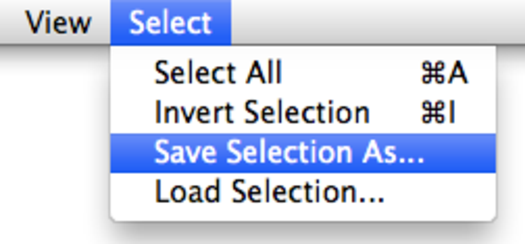
\includegraphics[width=0.5\textwidth]{3d_merge_save_selection.pdf}
		\caption{In the Select menu selection can be stored and loaded. This can be helpful during the \textit{Merge Once}  and \textit{Refine Once} runs.}
		\label{fig:3d_merge_save_selection}
	\end{figure}
	\item Merge the selected images all to one common 3D reference through \textit{Merge Once}\index{Merge Once!3D}, but with a \textit{Resolution of the merged dataset for the reference} set to 15 \AA.
	\item Now refine the alignment of the tilted images through the \textit{Refine Once} script, but with a smaller \textit{Stepsize of the phase origin search} while reducing \textit{zstarwin}.
	\item After the refinement have a look at the phase residual (\textit{MergePhaseRes}) for every refined image. If the phase residual is high it could have its origin in the CTF correction with a false defocus. This can be detected by verifying the merged data set. Because the data from most images will be complete up to 15 \AA~one can profit from the redundancy in the number of reflections to identify errors in the CTF correction. The defocus in the images, where the errors were detected has to be adjusted before proceeding with the refinement. 
	\item If the cause of the bad phase residual was not the CTF correction, check if refining the tilt geometry can improve the alignment. This would be done in another \textit{Merge\&Refine (Iterative)} run while having the parameter \textit{Refine Tilt Geometry (Only in 3D mode)}\index{Refine Tilt Geometry (Only in 3D mode)} set to Yes. This should only be done if a thorough reference already exist. You will discover that if the reference is not sufficient most commonly the tilt refinement will cause the tilt angle of all the refined images to increase.
	\item While running \textit{Merge\&Refine (Iterative)} with a reduced \textit{zstarwin} e.g. 0.1 and a smaller step size (0.5) one should have a look in the Images panel, where several output files appear. Glancing through the list you will discover that we have now created lattice lines. The first lattice line file in the processing workflow is named \textit{Latline after prescal}. It consists of the already known reflections with the index $(h,k,z^*)$, but in contrast to the  \textit{merge.aph} the amplitudes are CTF corrected and the intensity values coming from the same micrograph are scaled  by the program \texttt{latlineprescal}\index{latlineprescal}. Of more interest is the file \textit{Lattice Line fit data}. The difference of the reflections in this file compared to the previous one is apparent when looking at the $z^*$ values. In contrast to the randomly spaced $z^*$ values they are now equidistant. Because the program \texttt{latline} has fitted sinc functions to the measured data.   This can be seen as an interpolation of the data along the lattice lines. The lattice line fitting can be tuned by the bin size defined by the processing parameter \textit{3D: Bin-size for gathering data for the first lattice line guess (BINSIZ)}. You can verify the fitting outcome in the file \textit{PS: Lattice lines}\index{PS: Lattice lines} in the images panel. For both amplitude and phases you should have a smooth curve fitted through the data points given for every lattice line as in \autoref{fig:lattice_line_fit}. 
	
		\begin{figure}[H]
		\centering
		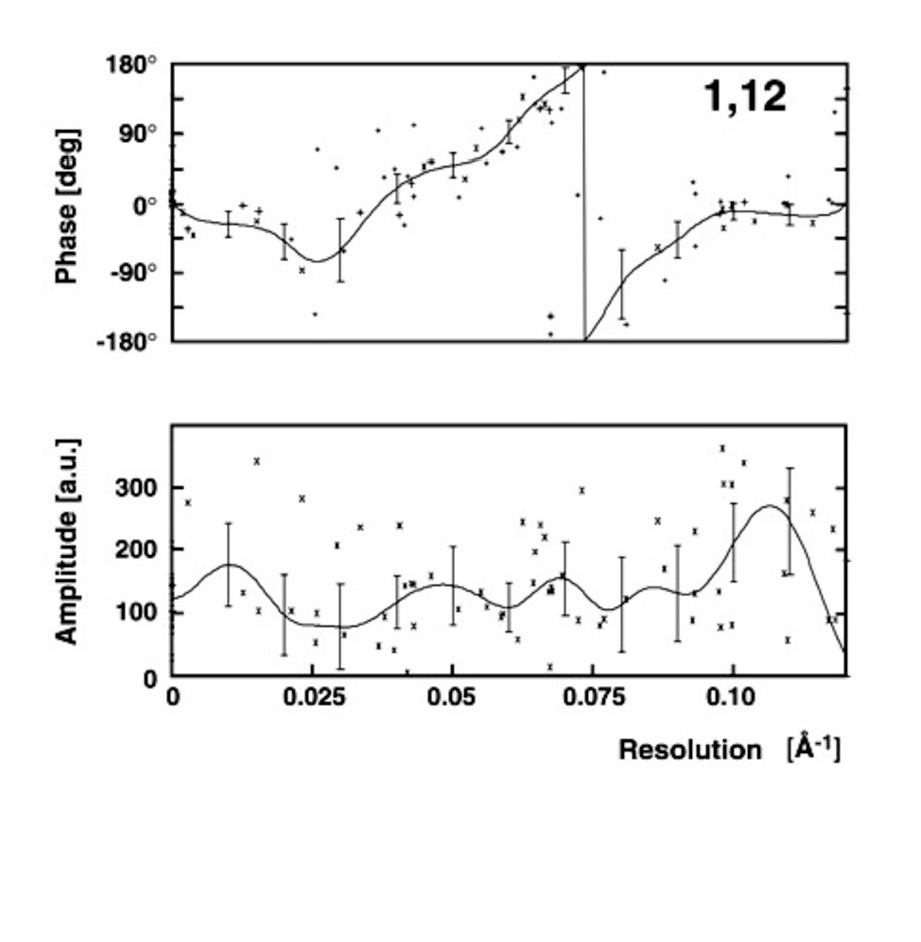
\includegraphics[width=0.8\textwidth]{lattice_line_fit.pdf}
		\caption{The lattice lines are created by fitting sinc functions to the measured data points. The fit can be inspected \textit{PS: Lattice lines}. Here the lattice line (1,12) is shown.}
		\label{fig:lattice_line_fit}
	\end{figure}
	
	\item After the first lattice line fit you should merge the refined data again but to a higher resolution with the \textit{Merge Once} script. You could therefore increase the parameter \textit{Merigning resolution limit} or you could also use the individual image resolution limits by changing the switch for \textit{Merging Resolution limit}. Asses the phases statistics of the high resolution reflections.
	\item If you find that your image data has a resolution of 5 \AA~or higher you should refine the beam tilt at this stage. This can be achieved by setting enabling the option \textit{Refine Beam Tilt}\index{Refine Beam Tilt} in the \textit{Merging Refinement} section for the refinement.
	\item Now you can include images of higher tilt and align them to your 3D reference with the \textit{Refine Once} script. The procedure of the refinement is done as before, so you should redo all the steps from \autoref{sec:refine_once_3d} to here. Remember that you can now decrease the parameter \textit{zstarwin}.
	\item The benefit of data stemming from sample tilted more than 25\textdegree  is that the tilt geometry is more trustworthy, since it was determined by lattice distortions through \texttt{emtilt}. This means when you have merged a fair amount of  higher tilt data you can in turn refine the tilt geometry of the lower tilt data.
	\item Once all image data has been included and all refinements have been done you can decide on the final resolution cut-off for the individual images \textit(Upper Resolution Limit) and run \textit{Final Merge}\index{Final Merge}.
	\item An important file that appears in the Images panel during merging is \textit{PS: TLTPLOT file}. This shows you the completeness of your 3D data set and allows you to determine at what tilt angle more data is needed for an even sampling of the 3D Fourier space.
	\item The final step in the 3D reconstruction of your structure is the calculation of the 3D map. This can be achieved with the \textit{Generate Merged Map}\index{Generate Merged Map} script. This creates a volume in CCP4 format named \textit{MAP: Final 3D Volume}. You can examine the result in Chimera by double-clicking it. With the example data set of GlpF the 3D map reconstruction should look similar to \autoref{fig:3d_map}
	
	\begin{figure}[H]
		\centering
		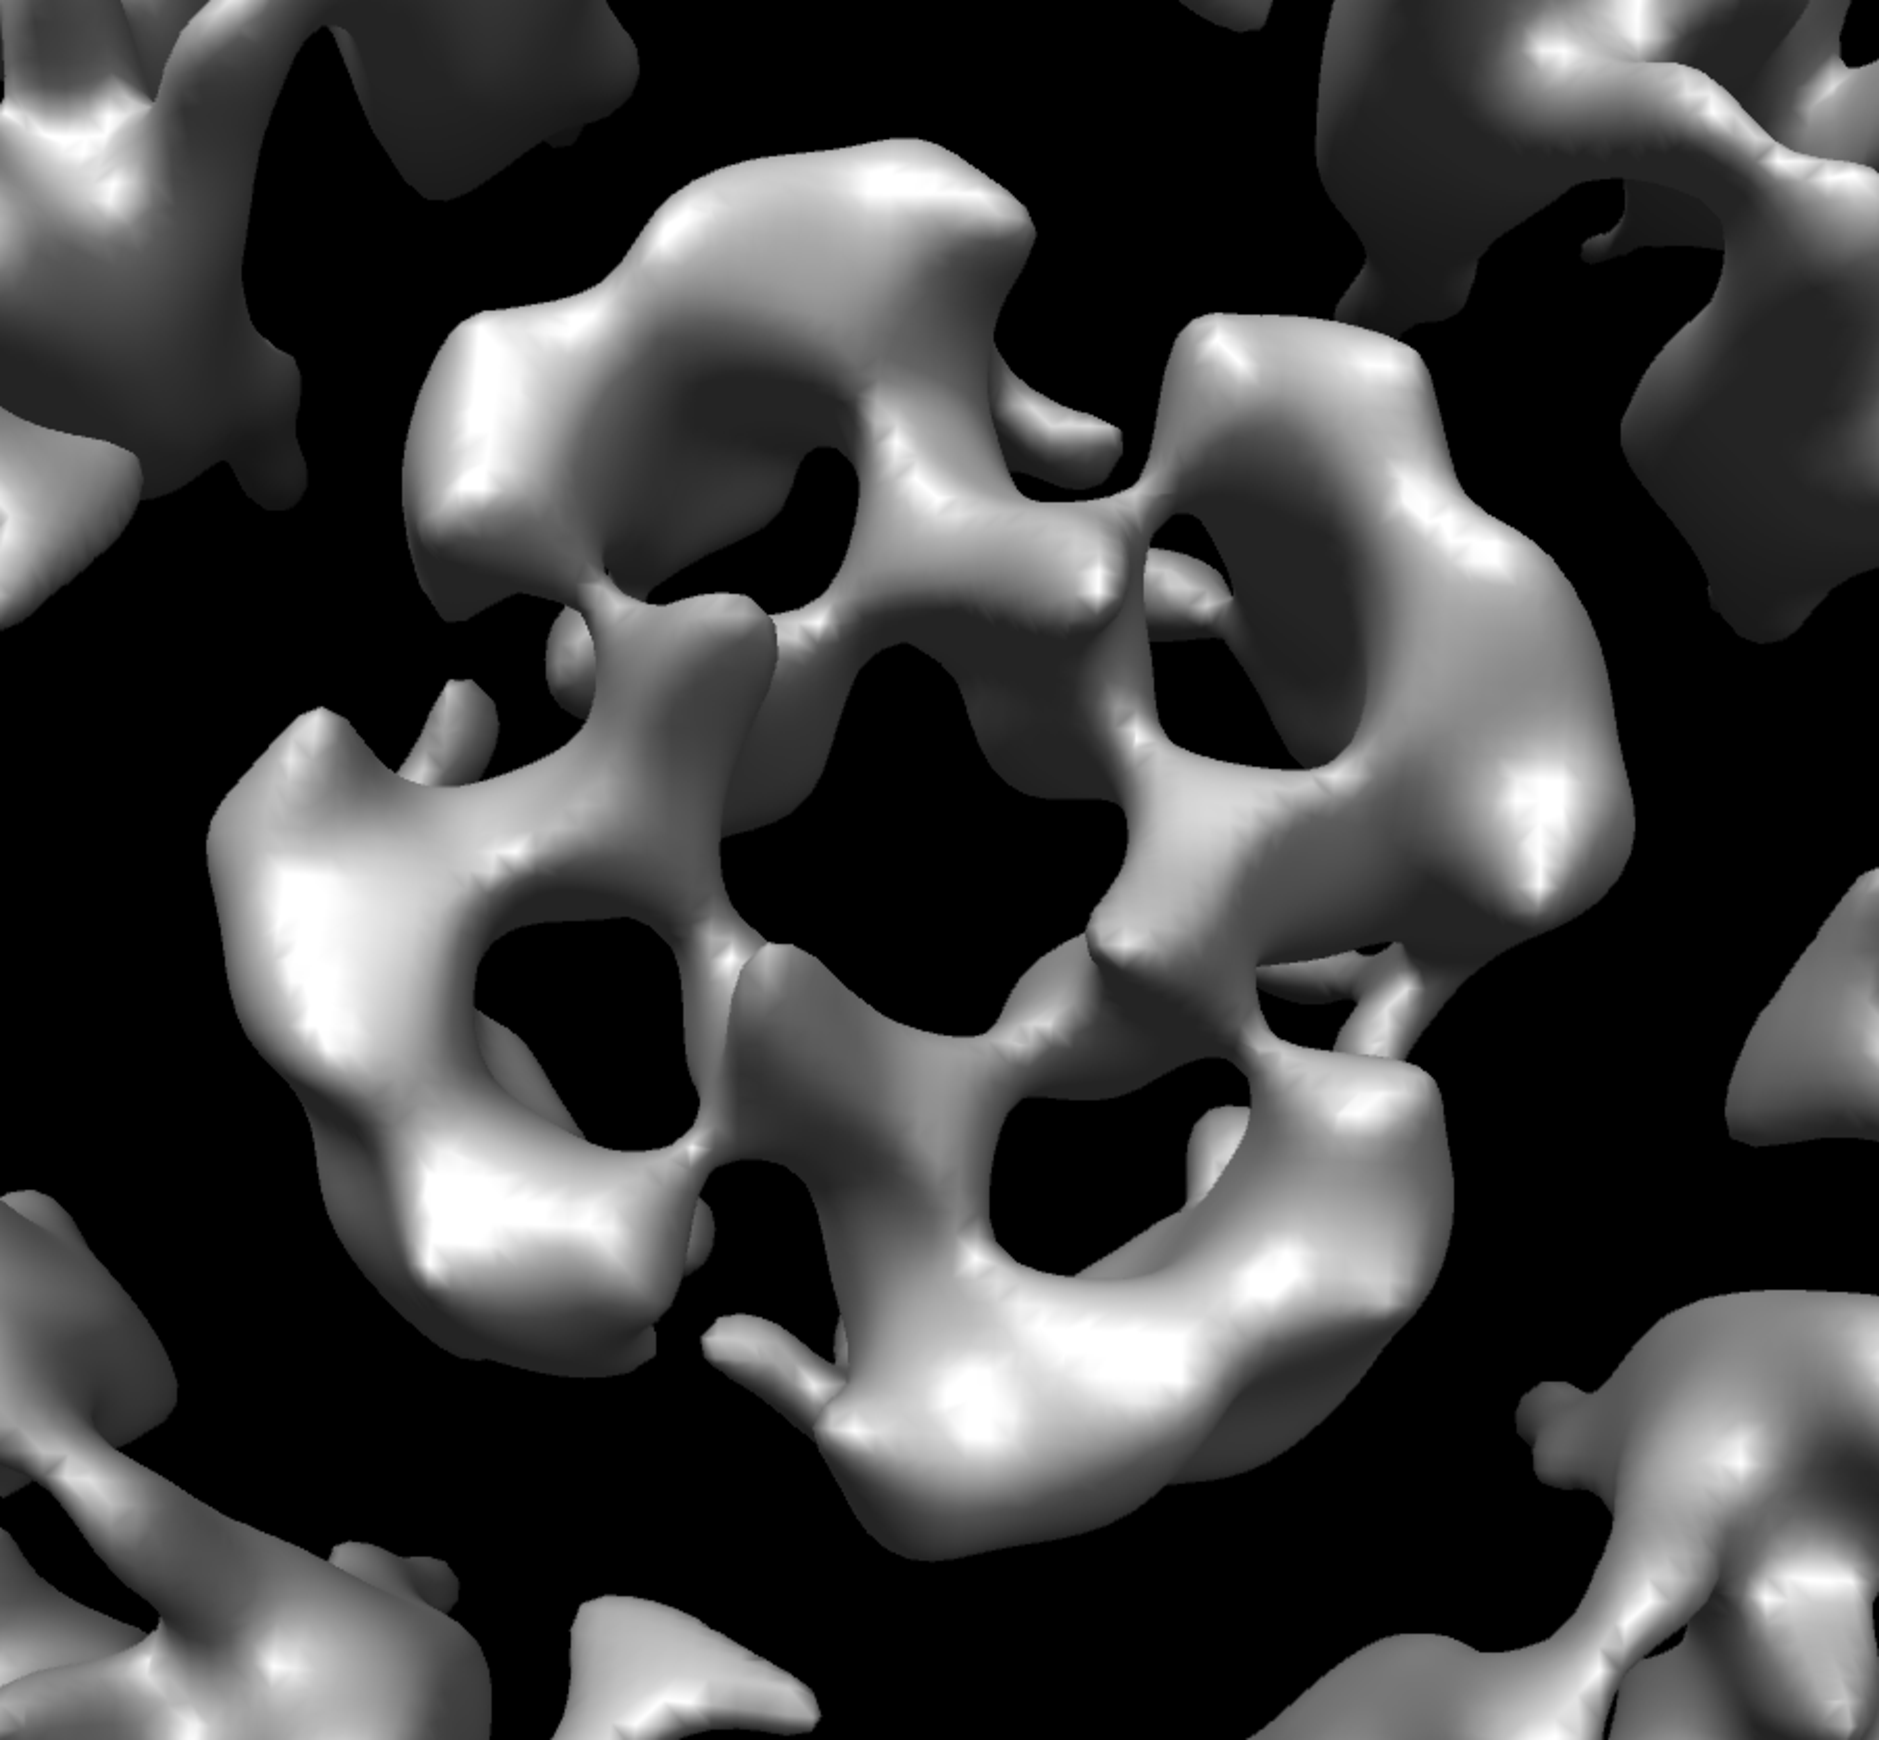
\includegraphics[width=0.8\textwidth]{3d_map.pdf}
		\caption{The 3D volume of the GlpF example data set.}
		\label{fig:3d_map}
	\end{figure}
	\item Once a reliable 3D-model has been generated on can re-process the already used images with the \textit{(Re-)Process all images} script. Thereby one can improve the data from the individual image data by unbending with a reference created through back projection from the model. We call this procedure synthetic unbending and it is described in \autoref{sec:syn_unbending}.
	
\end{enumerate}


